% .9 done on index contents
\chapter{Computation}

The only thing that's reliable is the definition. The only linkage or the connection is the reuse of the definition.

There are only two types of information: data and function. while we can consider function as a piece of data. and the third one is introduced as abstraction  

% Introduction
\chapter{Problems}

% introduction
\section{Problems}

To define a problem is defining a class at the same time.

To understand a problem is to know how to check whether one solution is correct or not.
\subsection{Verifying versus Searching}


% types of problems
\section{Types of Problems}
\subsection{Computational Problems}
\subsection{Learning Problems}
\subsection{Generic Problems}

% definition and properties of techniques
\section{Techniques}
The Classification of Techniques is a core concept in daily life.
\begin{figure}
  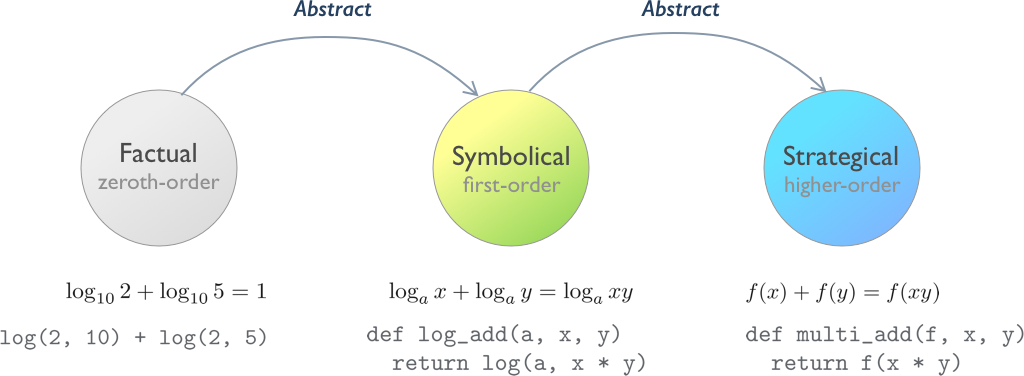
\includegraphics[width=\linewidth]{img/abstract-levels.png}
  \caption{Abstraction Levels}
  \label{fig:abstract-levels}
\end{figure}
\subsection{Robustness of Techniques}
\subsection{Frequency of Usage}
\subsection{Ad-Hoc versus Generic}
One phenominon that I experience a lot is the way people don't distinguish the difference between a ad-hoc technique and a generic technique. When a teacher or a guy present a way to solve a specific problem, few people will appreciate the robustness of this technique, that how well can you transfer your ability on this learning to another situations. But because of their inability to distinguish hardness and robustness, that leads to a dangerous place, that you have to learn too much techniques to cope with every problems, but you don't have enough time for learning these. And the teacher may think by doing an ad-hoc problem will lead to a better understanding for a more generic solving ability, which is vague. You don't learn too much on ad-hoc problems. You only know how to solve it in a nearby situations. The overall hint on a more generic solving strategies are often weak to recognize.

People don't know how to appreciate the robustness of techniques. Only can they find the dramatic changes of events. Even you simply press the button, you believe the underlining changes belongs to your smartness, well the main reason is the engineering behind the scene to smooth the user experience.
\subsection{Intensity of Signal}
\subsection{Trainability of Techniques}
Both the solving radius and the applicability.

% types of techniques
\section{Types of Techniques}
\subsection{Factual Techniques}
\subsection{Algorithmic Techniques}
\subsection{Strategic Techniques}
\subsection{Generic Techniques}
\subsection{Expansion Techniques}


% Definition
% \section{Replaceable Definition}
\subsection{Reference and Dereference}

% Composition
\section{Composition}
% \subsection{Array and String}
% \subsection{Hash Object}

% Transformation
\section{Transformation}

One thing I have to remember is that you have to make the instruction work for all instant. This is the foundation of this book. You have to make abstraction before you make transformation.

The transformation you define is for all not for instance. Even in turing machine, you move left twice, you don't care about the one you missed, because that is not what you care, no matter what symbol is on that square, it's the same instruction. This is the abstraction of operation, on operation to deal with all situations.

What intuitive really means is the automatic autocorrection based on the event trasnformational rules in brains, that processed in the subconscious. And the stregth of the neurons is how intuitive it will be.
\subsection{Events}

The first three are from an article by Chaitin\cite{chaitin}.

% \begin{figure}
%   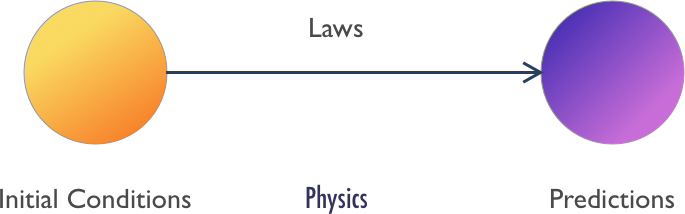
\includegraphics[width=\linewidth]{img/physics.png}
%   \caption{Computation Models}
%   \label{fig:phyics}
% \end{figure}
%
% \begin{figure}
%   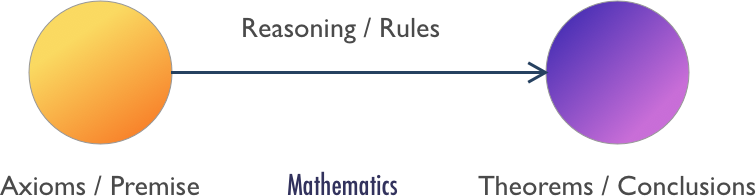
\includegraphics[width=\linewidth]{img/math.png}
%   \caption{Computation Models}
%   \label{fig:math}
% \end{figure}
%
% \begin{figure}
%   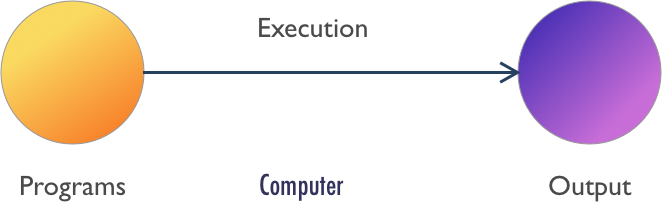
\includegraphics[width=\linewidth]{img/computer.png}
%   \caption{Computation Models}
%   \label{fig:computer}
% \end{figure}

% \[
%   \text{Theory}\xrightarrow{\displaystyle \text{Calculations}}\text{Predictions for Observations}
% \]
%
% \[
%   \text{Axioms}\xrightarrow{\displaystyle \text{Reasoning}}\text{Theorems}
% \]
%
% \[
%   \text{Program}\xrightarrow{\displaystyle \text{Execution on Computer}}\text{Output}
% \]
%
%
% \[
%   \text{Premise}\xrightarrow{\displaystyle \text{Rules}}\text{Conclusions}
% \]

\begin{figure}
  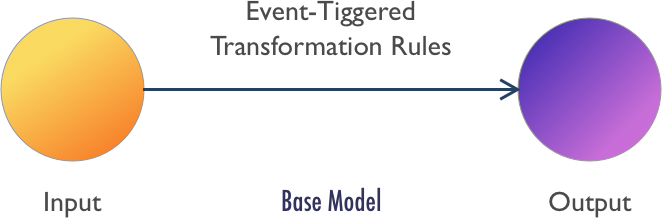
\includegraphics[width=\linewidth]{img/base.png}
  \caption{Computation Models}
  \label{fig:base}
\end{figure}

The rules mean under what conditions do what.

By saying conditions, first you have to know how to recognize conditions and what is recognizable conditions, of course that's when you definable, which in turn means distinguishable.

By saying doing, that means you have to know what is allow to transform.

\begin{figure}
  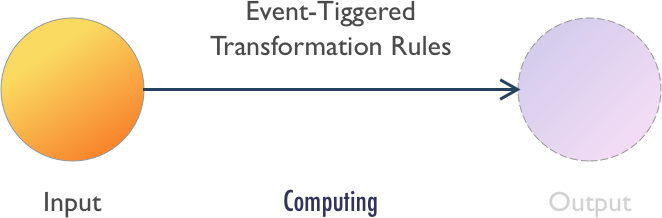
\includegraphics[width=\linewidth]{img/computing.png}
  \caption{Schematic Definition of Computation}
  \label{fig:computation}
\end{figure}

If we have clearly defined the \textbf{computing} procedure, we can easily compute. That means the input is distinguishable from others and the transformation rule is clear and distinguishable.
For example:
\begin{verbatim}
  def add(x)
    return x + 1
\end{verbatim}

And your goal is to compute:

\begin{verbatim}
  add(3)
\end{verbatim}

\begin{figure}
  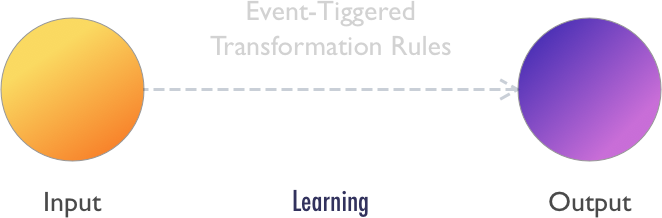
\includegraphics[width=\linewidth]{img/learning.png}
  \caption{Schematic Definition of Learning}
  \label{fig:learning}
\end{figure}

Whereas \textbf{learning} is that you know the input and output, but you don't know the transformation rules.

For example:
\begin{verbatim}
  add(3) = 4
  add(4) = 5
  add(5) = 6
  add(6) = 7
\end{verbatim}

And your goal is to compute:

\begin{verbatim}
  add(10)
\end{verbatim}

\begin{figure}
  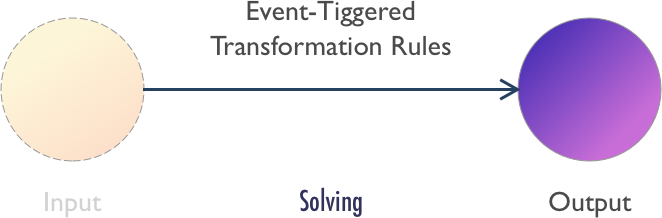
\includegraphics[width=\linewidth]{img/solving.png}
  \caption{Schematic Definition of Solving}
  \label{fig:solving}
\end{figure}

\textbf{Searching} is to find an instance which satisfies certain criteria in terms of computing algorithm.

For example:
\begin{verbatim}
  def add(x)
    return x + 1
  add(m) = 5
\end{verbatim}

And your goal is to compute:

\begin{verbatim}
  m
\end{verbatim}

\subsection{Inputs and Outputs}
% \subsection{Benefits of Event-Based View}

% Computation
\chapter{Problems}

% introduction
\section{Problems}

To define a problem is defining a class at the same time.

To understand a problem is to know how to check whether one solution is correct or not.
\subsection{Verifying versus Searching}


% types of problems
\section{Types of Problems}
\subsection{Computational Problems}
\subsection{Learning Problems}
\subsection{Generic Problems}

% definition and properties of techniques
\section{Techniques}
The Classification of Techniques is a core concept in daily life.
\begin{figure}
  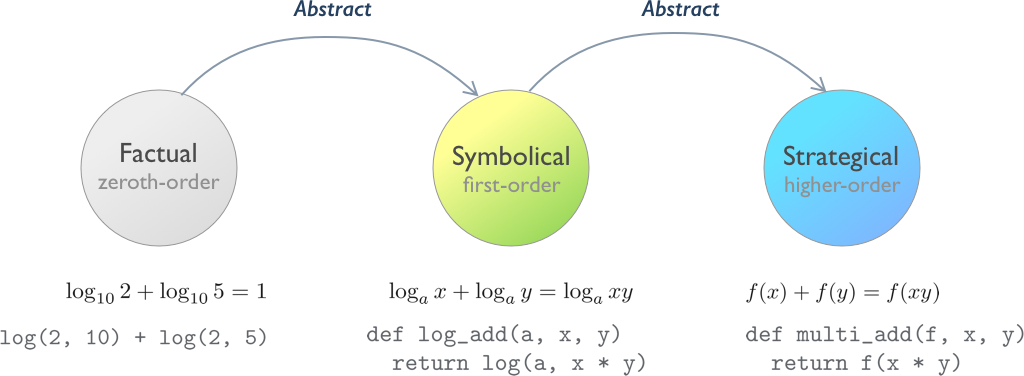
\includegraphics[width=\linewidth]{img/abstract-levels.png}
  \caption{Abstraction Levels}
  \label{fig:abstract-levels}
\end{figure}
\subsection{Robustness of Techniques}
\subsection{Frequency of Usage}
\subsection{Ad-Hoc versus Generic}
One phenominon that I experience a lot is the way people don't distinguish the difference between a ad-hoc technique and a generic technique. When a teacher or a guy present a way to solve a specific problem, few people will appreciate the robustness of this technique, that how well can you transfer your ability on this learning to another situations. But because of their inability to distinguish hardness and robustness, that leads to a dangerous place, that you have to learn too much techniques to cope with every problems, but you don't have enough time for learning these. And the teacher may think by doing an ad-hoc problem will lead to a better understanding for a more generic solving ability, which is vague. You don't learn too much on ad-hoc problems. You only know how to solve it in a nearby situations. The overall hint on a more generic solving strategies are often weak to recognize.

People don't know how to appreciate the robustness of techniques. Only can they find the dramatic changes of events. Even you simply press the button, you believe the underlining changes belongs to your smartness, well the main reason is the engineering behind the scene to smooth the user experience.
\subsection{Intensity of Signal}
\subsection{Trainability of Techniques}
Both the solving radius and the applicability.

% types of techniques
\section{Types of Techniques}
\subsection{Factual Techniques}
\subsection{Algorithmic Techniques}
\subsection{Strategic Techniques}
\subsection{Generic Techniques}
\subsection{Expansion Techniques}


% CTT
\subsection{Boundary of Computation}
\subsection*{Turing Completeness}

What I guess is that the reason of the robustness of Turing machine is that it can simulation any well-defined thought, the distinguishability at its highest level. No ambiguity is allowed. Everything you can distinguish clearly can be represented in the system. Every rule you can say precisely can be emulated in the machine. Every transformation  every possible computation is within the power of a Turing machine.
% \subsection{Turing Machine and $\lambda$-Calculus}
\subsubsection*{Church-Turing Thesis}

The Turing machine are capable of doing following abilities:

1. store and retrive data.
2. transform  data to another one.
3. able to compute in a sequencial order.
4. able to jump to a specific instruction position.

\chapter{Problems}

% introduction
\section{Problems}

To define a problem is defining a class at the same time.

To understand a problem is to know how to check whether one solution is correct or not.
\subsection{Verifying versus Searching}


% types of problems
\section{Types of Problems}
\subsection{Computational Problems}
\subsection{Learning Problems}
\subsection{Generic Problems}

% definition and properties of techniques
\section{Techniques}
The Classification of Techniques is a core concept in daily life.
\begin{figure}
  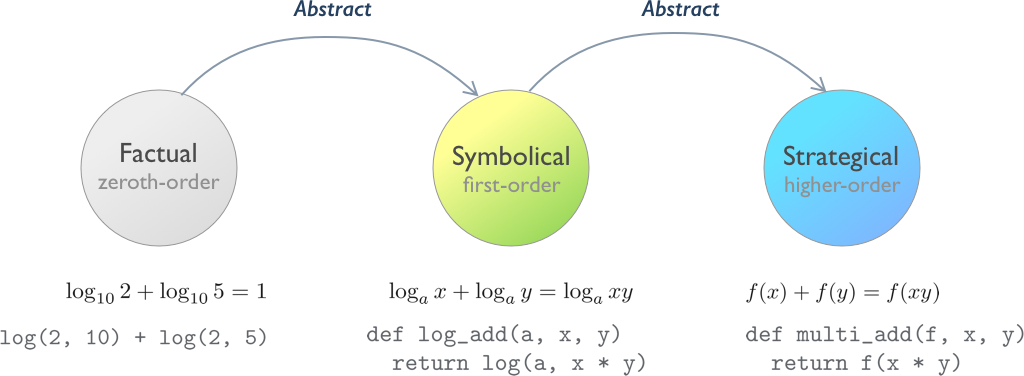
\includegraphics[width=\linewidth]{img/abstract-levels.png}
  \caption{Abstraction Levels}
  \label{fig:abstract-levels}
\end{figure}
\subsection{Robustness of Techniques}
\subsection{Frequency of Usage}
\subsection{Ad-Hoc versus Generic}
One phenominon that I experience a lot is the way people don't distinguish the difference between a ad-hoc technique and a generic technique. When a teacher or a guy present a way to solve a specific problem, few people will appreciate the robustness of this technique, that how well can you transfer your ability on this learning to another situations. But because of their inability to distinguish hardness and robustness, that leads to a dangerous place, that you have to learn too much techniques to cope with every problems, but you don't have enough time for learning these. And the teacher may think by doing an ad-hoc problem will lead to a better understanding for a more generic solving ability, which is vague. You don't learn too much on ad-hoc problems. You only know how to solve it in a nearby situations. The overall hint on a more generic solving strategies are often weak to recognize.

People don't know how to appreciate the robustness of techniques. Only can they find the dramatic changes of events. Even you simply press the button, you believe the underlining changes belongs to your smartness, well the main reason is the engineering behind the scene to smooth the user experience.
\subsection{Intensity of Signal}
\subsection{Trainability of Techniques}
Both the solving radius and the applicability.

% types of techniques
\section{Types of Techniques}
\subsection{Factual Techniques}
\subsection{Algorithmic Techniques}
\subsection{Strategic Techniques}
\subsection{Generic Techniques}
\subsection{Expansion Techniques}

